\documentclass{beamer}
\mode<presentation>
\usepackage{amsmath}
\usepackage{amssymb}
%\usepackage{advdate}
\usepackage{adjustbox}
\usepackage{subcaption}
\usepackage{enumitem}
\usepackage{multicol}
\usepackage{mathtools}
\usepackage{listings}
\usepackage{float}
\usepackage{graphicx}
\usepackage{url}
\def\UrlBreaks{\do\/\do-}
\usetheme{Boadilla}
\usecolortheme{lily}
\setbeamertemplate{footline}
{
  \leavevmode%
  \hbox{%
  \begin{beamercolorbox}[wd=\paperwidth,ht=2.25ex,dp=1ex,right]{author in head/foot}%
    \insertframenumber{} / \inserttotalframenumber\hspace*{2ex} 
  \end{beamercolorbox}}%
  \vskip0pt%
}
\setbeamertemplate{navigation symbols}{}

\providecommand{\nCr}[2]{\,^{#1}C_{#2}} % nCr
\providecommand{\nPr}[2]{\,^{#1}P_{#2}} % nPr
\providecommand{\mbf}{\mathbf}
\providecommand{\pr}[1]{\ensuremath{\Pr\left(#1\right)}}
\providecommand{\qfunc}[1]{\ensuremath{Q\left(#1\right)}}
\providecommand{\sbrak}[1]{\ensuremath{{}\left[#1\right]}}
\providecommand{\lsbrak}[1]{\ensuremath{{}\left[#1\right.}}
\providecommand{\rsbrak}[1]{\ensuremath{{}\left.#1\right]}}
\providecommand{\brak}[1]{\ensuremath{\left(#1\right)}}
\providecommand{\lbrak}[1]{\ensuremath{\left(#1\right.}}
\providecommand{\rbrak}[1]{\ensuremath{\left.#1\right)}}
\providecommand{\cbrak}[1]{\ensuremath{\left\{#1\right\}}}
\providecommand{\lcbrak}[1]{\ensuremath{\left\{#1\right.}}
\providecommand{\rcbrak}[1]{\ensuremath{\left.#1\right\}}}
\theoremstyle{remark}
\newtheorem{rem}{Remark}
\newcommand{\sgn}{\mathop{\mathrm{sgn}}}
\providecommand{\abs}[1]{\left\vert#1\right\vert}
\providecommand{\res}[1]{\Res\displaylimits_{#1}} 
\providecommand{\norm}[1]{\lVert#1\rVert}
\providecommand{\mtx}[1]{\mathbf{#1}}
\providecommand{\mean}[1]{E\left[ #1 \right]}
\providecommand{\fourier}{\overset{\mathcal{F}}{ \rightleftharpoons}}
%\providecommand{\hilbert}{\overset{\mathcal{H}}{ \rightleftharpoons}}
\providecommand{\system}{\overset{\mathcal{H}}{ \longleftrightarrow}}
	%\newcommand{\solution}[2]{\textbf{Solution:}{#1}}
%\newcommand{\solution}{\noindent \textbf{Solution: }}
\providecommand{\dec}[2]{\ensuremath{\overset{#1}{\underset{#2}{\gtrless}}}}
\newcommand{\myvec}[1]{\ensuremath{\begin{pmatrix}#1\end{pmatrix}}}
\let\vec\mathbf

\lstset{
language=C,
frame=single, 
breaklines=true,
columns=fullflexible
}

\numberwithin{equation}{section}

\title{Presentation - Matgeo}
\author{Aryansingh Sonaye \\
AI25BTECH11032 \\
EE1030 - Matrix Theory}

\date{\today} 
\begin{document}

\begin{frame}
\titlepage
\end{frame}

\section{Problem}
\begin{frame}
\frametitle{Problem Statement}
\textbf{Problem 4.12.46 :}\\
Find the values of $\theta$ and $p$, if the equation
\begin{align}
x\cos\theta + y\sin\theta &= p
\end{align}
is the normal form of the line
\begin{align}
\sqrt{3}x + y + 2 &= 0.
\end{align}
\end{frame}

\section{Solution}
\subsection{Description of Variables used}
\begin{frame}
\frametitle{Description of Variables used}
\begin{table}[H]
\centering
\begin{tabular}{|c|c|}
\hline
\textbf{Quantity} & \textbf{Value} \\
\hline
Normal vector $\vec{n}$ & $\myvec{\sqrt{3} \\ 1}$ \\
\hline
Constant $c$ & $2$ \\
\hline
\end{tabular}
\caption{}
\label{}
\end{table}


\end{frame}

\subsection{Theoretical Solution }
\begin{frame}
\frametitle{Theoretical Solution}
\noindent The line can be expressed as
\begin{align}
\vec{n}^T \vec{u} &= -c. \label{eq1}
\end{align}

The length of the normal is
\begin{align}
\|\vec{n}\| &= \sqrt{(\sqrt{3})^2 + 1^2} = 2. \label{eq2}
\end{align}

Thus, the unit normal becomes
\begin{align}
\hat{\vec{n}} &= \frac{\vec{n}}{\|\vec{n}\|} 
= \myvec{\tfrac{\sqrt{3}}{2} \\[4pt] \tfrac{1}{2}}. \label{eq3}
\end{align}
\end{frame}

\begin{frame}
\frametitle{Theoretical Solution}
Dividing (3) by $\|\vec{n}\|$ gives the normal form:
\begin{align}
\hat{\vec{n}}^T \vec{u} &= \frac{-c}{\|\vec{n}\|} = -1. \label{eq4}
\end{align}

Comparing with the standard normal form
\begin{align}
x\cos\theta\, + y\sin\theta\, &= p,
\end{align}
we identify
\begin{align}
\cos\theta &= \tfrac{\sqrt{3}}{2}, \quad 
\sin\theta = \tfrac{1}{2}. \label{eq5}
\end{align}

Hence,
\begin{align}
\theta &= \tfrac{\pi}{6}, \quad p = -1. \label{eq6}
\end{align}

\noindent \textbf{Final Answer: } 
\begin{align}
\boxed{
\theta = \tfrac{\pi}{6}, \quad p = -1.
}
\end{align}

\end{frame}







\subsection{Plot}
\begin{frame}
    \frametitle{Plot}
\begin{figure}[H]
   \centering
   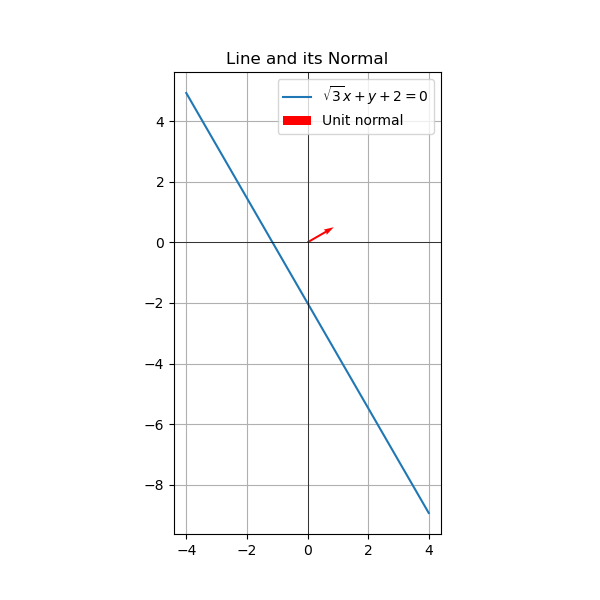
\includegraphics[width=0.7\columnwidth]{figs/normalform.png}
   \caption{}
   \label{}
   \end{figure}
\end{frame}

\begin{frame}[fragile]
    \frametitle{Code - C}
    \begin{lstlisting}
#include <stdio.h>
#include <math.h>

// Compute norm of a 2D vector
double norm(double *vec) {
    return sqrt(vec[0]*vec[0] + vec[1]*vec[1]);
}

// Normalize a 2D vector
void normalize(double *vec, double *out) {
    double n = norm(vec);
    out[0] = vec[0]/n;
    out[1] = vec[1]/n;
}

    \end{lstlisting}
    \end{frame}

    \begin{frame}[fragile]
    \frametitle{Code - C}
    \begin{lstlisting}

// Compute p = -c / norm(n)
double compute_p(double *vec, double c) {
    double n = norm(vec);
    return -c / n;
}

\end{lstlisting}
\end{frame}

\begin{frame}[fragile]
    \frametitle{Code - Python(with shared C code)}
    The code to obtain the required plot is
    \begin{lstlisting}

import ctypes
import numpy as np
import matplotlib.pyplot as plt

# Load shared library
lib = ctypes.CDLL("./liblineutils.so")

# Define argument/return types
lib.norm.argtypes = [ctypes.POINTER(ctypes.c_double)]
lib.norm.restype = ctypes.c_double

lib.normalize.argtypes = [ctypes.POINTER(ctypes.c_double), ctypes.POINTER(ctypes.c_double)]
lib.normalize.restype = None

\end{lstlisting}
\end{frame}
\begin{frame}[fragile]
\frametitle{Code - Python(with shared C code)}
\begin{lstlisting}
lib.compute_p.argtypes = [ctypes.POINTER(ctypes.c_double), ctypes.c_double]
lib.compute_p.restype = ctypes.c_double

# Input data
n = np.array([np.sqrt(3), 1.0], dtype=np.double)
c = 2.0

# Allocate output for unit normal
unit_n = np.zeros(2, dtype=np.double)

# Convert numpy array to C pointer
n_ptr = n.ctypes.data_as(ctypes.POINTER(ctypes.c_double))
unit_ptr = unit_n.ctypes.data_as(ctypes.POINTER(ctypes.c_double))

\end{lstlisting}
\end{frame}

\begin{frame}[fragile]
\frametitle{Code - Python(with shared C code)}
\begin{lstlisting}

# Call C functions
norm_val = lib.norm(n_ptr)
lib.normalize(n_ptr, unit_ptr)
p_val = lib.compute_p(n_ptr, c)

print("||n|| =", norm_val)
print("Unit normal =", unit_n)
print("p =", p_val)

# ----------------- Plotting -----------------
# Line: sqrt(3)x + y + 2 = 0  => y = -sqrt(3)x - 2
x_vals = np.linspace(-4, 4, 200)
y_vals = -np.sqrt(3)*x_vals - 2


\end{lstlisting}
\end{frame}

\begin{frame}[fragile]
\frametitle{Code - Python(with shared C code)}
\begin{lstlisting}
#Call C functions
norm_val = lib.norm(n_ptr)
lib.normalize(n_ptr, unit_ptr)
p_val = lib.compute_p(n_ptr, c)

print("||n|| =", norm_val)
print("Unit normal =", unit_n)
print("p =", p_val)

# ----------------- Plotting -----------------
# Line: sqrt(3)x + y + 2 = 0  => y = -sqrt(3)x - 2
x_vals = np.linspace(-4, 4, 200)
y_vals = -np.sqrt(3)*x_vals - 2
# Normal vector (scaled for plotting)
origin = np.array([0,0])
normal_line = np.vstack([origin, unit_n*2])  # scale for visibility

\end{lstlisting}
\end{frame}

\begin{frame}[fragile]
\frametitle{Code - Python(with shared C code)}
\begin{lstlisting}
plt.figure(figsize=(6,6))
plt.plot(x_vals, y_vals, label=r"$\sqrt{3}x+y+2=0$")
plt.quiver(0,0, unit_n[0], unit_n[1], angles='xy', scale_units='xy', scale=1, color='red', label="Unit normal")

plt.axhline(0, color='black', linewidth=0.5)
plt.axvline(0, color='black', linewidth=0.5)
plt.legend()
plt.gca().set_aspect("equal")
plt.title("Line and its Normal")
plt.grid(True)
plt.savefig("normalform.png")
plt.show()

\end{lstlisting}
\end{frame}


\begin{frame}[fragile]
\frametitle{Code - Python only}
\begin{lstlisting}
import numpy as np
import matplotlib.pyplot as plt

# Input
n = np.array([np.sqrt(3.0), 1.0])
c = 2.0

# Compute norm, unit normal, and p
norm_n = np.linalg.norm(n)
unit_n = n / norm_n
p = -c / norm_n
theta = np.arctan2(unit_n[1], unit_n[0])



\end{lstlisting}
\end{frame}
\begin{frame}[fragile]
\frametitle{Code - Python only}
\begin{lstlisting}
# Print results
print("n =", n)
print("c =", c)
print("||n|| =", norm_n)
print("unit normal =", unit_n)
print("p =", p)
print("theta =", theta, "rad (~", theta*180/np.pi, "degrees )")

# Plot the line: sqrt(3)x + y + 2 = 0 -> y = -sqrt(3)x - 2
x_vals = np.linspace(-4, 4, 400)
y_vals = -np.sqrt(3.0) * x_vals - 2

plt.figure(figsize=(6,6))
plt.plot(x_vals, y_vals, label="Line: sqrt(3)x + y + 2 = 0")


\end{lstlisting}
\end{frame}

\begin{frame}[fragile]
\frametitle{Code - Python only}
\begin{lstlisting}
# Plot unit normal arrow from origin
plt.quiver(0, 0, unit_n[0], unit_n[1],
           angles="xy", scale_units="xy", scale=1,
           color="red", label="Unit normal")

# Axes and labels
plt.axhline(0, color="black", linewidth=0.5)
plt.axvline(0, color="black", linewidth=0.5)
plt.gca().set_aspect("equal")
plt.xlim(-4, 4)
plt.ylim(-6, 4)
plt.legend()
plt.title("Line and its Unit Normal")
plt.grid(True)
plt.savefig("normalform_new.png")
plt.show()


\end{lstlisting}
\end{frame}

\end{document}
